\documentclass{hw}
\usepackage{mhchem}
\usepackage{nuc}
\usepackage{siunitx}
\usepackage{amsmath}
\usepackage{cancel}
\graphicspath{ {images/}}

\author{J.R. Powers-Luhn}
\date{2016/09/28}
\title{Homework \#4}

\begin{document}

\problem{}
Use the NIST ASTAR to find the range of a \SI{10}{\mega\electronvolt} alpha particle, and then use the range values at lower energies to determine at what depth a \SI{10}{\mega\electronvolt}/nucleon alpha particle has traveled 99\% of its range. Do the same for a \SI{20}{\mega\electronvolt}/nucleon alpha and \SI{50}{\mega\electronvolt}/nucleon alpha. Use this information for your semester stopping power assignment to help guide you in determining a lower energy limit/cutoff when calculating ranges.
\solution
\begin{centering}
\begin{table}[h]
	\begin{tabular}{c c c c}
		T & CSDA & 1\% CSDA & T$^\prime$ \\
		\hline
		\SI{10}{\mega\electronvolt} & \SI{1.13e-2}{\centi\meter} & \SI{1.13e-4}{\centi\meter} & \SI{7.00e-2}{\mega\electronvolt} \\
		\SI{40}{\mega\electronvolt} & \SI{1.240e-1}{\centi\meter} & \SI{1.240e-3}{\centi\meter} & \SI{2.25}{\mega\electronvolt} \\
		\SI{80}{\mega\electronvolt} & \SI{4.287e-1}{\centi\meter} & \SI{4.287e-3}{\centi\meter} & \SI{5.5}{\mega\electronvolt} \\
		\SI{200}{\mega\electronvolt} & \SI{2.240}{\centi\meter} & \SI{2.240e-2}{\centi\meter} & \SI{15}{\mega\electronvolt} \\
	\end{tabular}
	\caption{Estimated ranges after 99\% energy loss}\label{problem1}
\end{table}
\end{centering}
From ASTAR, a \SI{10}{\mega\electronvolt} $ \alpha $ particle travels \SI{1.13e-2}{\centi\meter} in water. At the time that it has travelled 99\% of this range, it has an energy of \SI{7e-2}{\mega\electronvolt}. Similar results are summarized in table \ref{problem1}


\problem{Anderson 4.2}
Use Eqution 4.13 to calculate the range of a \SI{5}{\mega\electronvolt} alpha particle in \ce{N_2} gas at \SI{760}{\mmHg} pressure. Assume that the exponential integral at $ T_1 $ (low-energy limit) and $ R_1(T_1) $ can be neglected.

\begin{align*}
	R &= \frac{M c^2 I^2}{32 z^2 \pi r_0^2 \left( m_e c^2 \right)^3 N_A \left(Z / M_m \right) \rho} \int^{u_0}_{u_1} \frac{du}{\ln u} + R_1 \left( T_1 \right) \\
	&= \frac{M c^2 I^2}{32 z^2 \pi r_0^2 \left( m_e c^2 \right)^3 N_A \left(Z / M_m \right) \rho} \left[ \text{Ei}\left(\ln u_0 \right) - \text{Ei}\left( \ln u_1 \right) \right] + R_1 \left( T_1 \right) \tag{4.13}
\end{align*}
with
\begin{equation}
	u = \left( \frac{4 m_e c^2 \tau}{I} \right)^2 = \left( \frac{4 m_e \cancel{c^2} T}{I M \cancel{c^2}} \right)^2
\end{equation}
\solution
See attached addendum for calculations.
\begin{center}
	R = 3.04
\end{center}

\problem{Anderson 4.5}
Calculate the ratio of the range of a \SI{14}{\mega\electronvolt} \ce{^{14}N^{+++}} ion to the range of a \SI{1}{\mega\electronvolt} proton. Use equation 4.18.

\begin{equation}
	\left( R \rho \right)_b \approx \frac{\left( M/z^2 \right)_b}{\left( M / z^2 \right)_a} \left( R \rho \right)_a \tag{4.18}
	\label{4.18}
\end{equation}
\solution
We know that for particles with similar values of $ \tau = T / m c^2 $, equation \ref{4.18} can be used to compare Range-density values. Therefore:
\begin{align*}
	\left( R \rho \right)_b &\approx \frac{\left( M/z^2 \right)_b}{\left( M / z^2 \right)_a} \left( R \rho \right)_a \\
	&\approx \frac{\left( 14/3^2 \right)_b}{\left( 1 / 1^2 \right)_a} \left( R \rho \right)_a \\
	&\approx 1.56 \left( R \rho \right)_a
\end{align*}
The \SI{14}{\mega\electronvolt} \ce{^{14}N^{+++}} ion will travel approximately \num{1.56} times further than the \SI{1}{\mega\electronvolt} proton.

\problem{}
Use the NIST PSTAR utility to do the following: produce a Bragg Curve for \SI{250}{\mega\electronvolt} protons passing through a variable water column, as measured by two air ionization chambers, each \SI{1}{\centi\meter} thick. Neglect energy loss in the ion chamber windows and in any air gaps between the ion chambers and water column. NIST states a \SI{250}{\mega\electronvolt} proton ranges out in about \SI{38}{\centi\meter} of water, so calculate the ratio of the ion chamber currents at \SIlist{0;10;20;30;35;36;37;38}{\centi\meter} of water between the ion chambers.

Assume dry air in the ion chambers at a density of \SI{0.0012}{\gram\per\centi\meter^3}. More details about this problem will be covered in class.
\solution
Calcluations are performed in the attached code. The curve produced is show in figure \ref{fig:bragg}

\begin{figure}[h]
	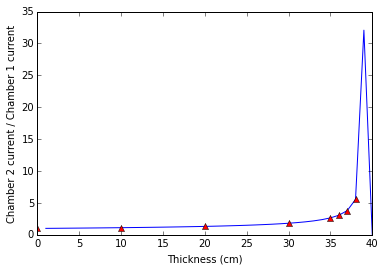
\includegraphics[width=15cm,height=10cm,keepaspectratio]{bragg}
	\caption{Bragg Curve for 250MeV proton in water}
	\label{fig:bragg}
\end{figure}

\end{document}